When dealing with a batch update comprising edge deletions $(u, v) \in \Delta^{t-}$ and insertions $(u, v) \in \Delta^{t+}$, if the total update size $|\Delta^{t-} \cup \Delta^{t+}|$ is relatively small compared to the total edge count $|E|$, only a small fraction of vertices are expected to undergo rank changes. To handle this, our earlier work proposed \textbf{Dynamic Frontier (DF)} and \textbf{Dynamic Frontier with Pruning (DF-P)} approaches, which employ an incremental process to identify affected vertices and update their ranks. Our research showed that DF/DF-P PageRank outperformed Static and Dynamic Traversal (DT) PageRank by $5.2\times$/$15.2\times$ and $1.3\times$/$3.5\times$\ignore{respectively} on real-world dynamic graphs, and by $7.2\times$/$9.6\times$ and $4.0\times$/$5.6\times$ on large graphs with random batch updates \cite{sahu2024df}.

Unfortunately, multicore CPUs have limited memory bandwidth and parallelism, making them unsuitable for graph algorithms like PageRank, which have a low computation-to-communication ratio. In contrast, GPUs offer high-bandwidth memory, connected in close proximity to thousands of lightweight cores with user-managed caches. Moreover, GPU hardware is designed to switch running threads at no cost to support memory access latency hiding. When appropriately designed, graph algorithms can significantly outperform CPU-based implementations on GPUs. This makes a GPU implementation of DF and DF-P PageRank attractive. In this section, we describe the design of DF and DF-P PageRank for GPUs.



\subsection{Design of Dynamic Frontier (DF) and Dynamic Frontier with Pruning (DF-P) PageRank for GPUs}
\label{sec:frontier}

\paragraph{Copying data to the device:}

A GPU has its own memory that supports a high volume of data transfers. Accordingly, we\ignore{first} copy the Compressed Sparse Row (CSR) representation of the current graph $G^t$, its transpose $G^{t\ (T)}$, the previous ranks of each vertex $R^{t-1}$, and the batch update consisting of edge deletions $\Delta^{t-}$ (both source and target vertex IDs in separate arrays) and edge insertions $\Delta^{t+}$ (source vertex IDs only). The CSR of $G^{t\ (T)}$ is used for computing PageRank scores, while that of $G^t$ is used for the initial and incremental marking of affected vertices. Note that we only need the source vertex IDs of edge insertions $(u, v) \in \Delta^{t+}$ as we only need to mark the outgoing neighbors of $u$ as affected. On the other hand, for edge deletions $(u, v) \in \Delta^{t-}$, we need both the source and target vertex IDs as we need to mark both the outgoing neighbors of $u$ and the target vertices of the edge deletions, i.e., $v$, as affected.

\paragraph{Partitioning vertices into low-degree and high-degree sets:}

Unlike threads on a multicore CPU, threads on a GPU are organized in hierarchy of warps, thread blocks, and grids. A warp consists of a group of threads that execute instructions is a fully synchronous manner, i.e., in lockstep. NVIDIA GPUs typically have a warp size of 32 threads. Further, a thread block consists of a group of threads which execute on the same Streaming Multiprocessor (SM) --- each warp in a thread block is executed in lockstep, and the SM schedules another warp in the thread block for execution, when one or more threads in the current warp are stalled (for example, due to a memory request). Since all threads in a thread block are executing on the same SM, they can readily communicate among themselves through a user-managed cache (also known as shared memory) that is private to each SM. Finally, a grid consists of a group of thread blocks, where each thread ...

We use a pair of kernels (functions executed on the GPU), i.e., a thread-per-vertex kernel and a block-per-vertex kernel, each for rank computation and incremental marking of affected vertices. A thread-per-vertex kernel is used to process low degree vertices, while a block-per-vertex kernel is used to process high-degree vertices. Using two different kernels allows us to improve processing performance for high-degree vertices, while minimizing resource wastage for low-degree vertices. For this, we partition the vertex IDs for the two kernels by their in-degree for the rank computation phase (the work to be performed by each thread is proportional to the in-degree of each vertex during the rank computation phase), and by their out-degree for the incremental marking of affected vertices (the work to be performed by each thread is proportional to the out-degree of each vertex during the incremental marking). This also helps minimize thread divergence with the thread-per-vertex kernel. The psuedocode for partitioning the vertices (by in- or out-degree of vertices) is given in Algorithm \ref{alg:partition}, with its explanation given in Section \ref{sec:partition}.

\paragraph{Marking the initial set of affected vertices:}

Upon each edge deletion $(u, v) \in \Delta^{t-}$ and edge insertion $(u, v) \in \Delta^{t+}$ in the batch update, with the DF and DF-P approaches, we need to mark the outgoing neighbors of vertex $u$ in both the prior snapshot $G^{t-1}$ and the current snapshot $G^t$ as affected. This is equivalent to marking the outgoing neighbors of $u$ for each edge deletion and insertion $(u, v) \in \Delta^{t-} \cup\Delta^{t+}$ as affected, and marking the target vertices of $v$ for each edge deletion $(u, v) \in \Delta^{t-}$ as affected. In order to achieve this, we use one kernel to the target vertices of $v$ for each edge deletion $(u, v) \in \Delta^{t-}$ as affected, and use a temporary array to indicate that the outgoing neighbors of $u$ for each edge deletion and insertion $(u, v) \in \Delta^{t-} \cup\Delta^{t+}$ need to be marked as affected later. A thread-per-vertex kernel and block-per-vertex kernel and then used to actually mark the outgoing neighbors of such vertices as affected. The vertex IDs between the two kernels are partitioned by out-degree (the work to be performed by each thread is proportional to the out-degree of each vertex during the marking), the thread divergence is expected to be minimal. Details of why this is done is given later.

\paragraph{Rank computation of each vertex, and incremental contraction of the set of affected vertices:}

We observe that, unlike on multicore CPUs, a synchronous implementation of the PageRank algorithm, which uses two separate rank vectors offers better performance than an asynchronous approach (which performs well on multicore CPUs). Accordingly, we use a synchronous implementation of the PageRank algorithm.

For the rank computation phase in each iteration, we use two different kernels --- a thread-per-vertex kernel for processing vertices with low in-degree, and a block-per-vertex kernel for processing high in-degree vertices. The thread-per-vertex kernel schedules one thread per vertex, and updated the rank of each vertex independently (in a sequential manner). On the other hand, the block-per-vertex kernels schedules a thread block per vertex, where each thread in a thread block computes the rank contribution of in-neighbors to the vertex in a strided fashion. These partial rank contributions are the written to shared memory, and a block reduce (sum) is performed to obtained the net rank contribution. The first thread in the thread block then updates rank of the given vertex. The vertex IDs between the two kernels are partitioned by in-degree (the work to be performed by each thread is proportional to the in-degree of each vertex during the rank computation phase), and hence, the thread divergence is expected to be minimal.

With the DF and DF-P approaches, if the relative change in the rank of a vertex $u$ is greater than the frontier tolerance $\tau_f$, we need to incrementally mark the outgoing neighbors $v \in G^t.out(u)$ of $u$ as affected \cite{sahu2024df}. However, performing this incremental marking during the rank computation phase may introduce significant thread divergence. This is because rank computation is performed using a thread-per-vertex and a block-per-vertex kernel, with the vertex IDs to be processed by each of the kernels being partitioned between the two by the in-degrees of the vertices, while the incremental marking of affected vertices need to processed by two similar kernels, with the vertex IDs being partitioned by their out-degree (the work to be performed by each thread is proportional to the out-degree of each vertex during the incremental marking) and not their in-degree. Since SMs execute warps in lockstep, this would mean that many threads would simply be waiting for the longest thread to complete, resulting is poor GPU utilization, and thus poor performance. Thus, for incremental marking of affected vertices, we simply use a temporary array to indicate that the neighbors of an vertex need to be incrementally marked as affected during rank computation. This can later be used with a pair of kernels to actually mark the outgoing neighbors of such vertices as affected.

With the DF-P approach, if the relative change in the rank of a vertex $u$ is within than the prune tolerance $\tau_p$, we need to mark the $u$ as not affected \cite{sahu2024df}. This is done directly unflagging it in the set of affected vertices, as it is $O(1)$ work, and does not introduce any significant thread divergence.

In the context of DF-P PageRank, vertices have the potential to be pruned, indicating that they are marked as not affected. Given the inclusion of a self-loop for each vertex in the graph (as discussed in Sections \ref{sec:dataset} and \ref{sec:batch-generation}), we utilize a closed-loop formula for computing the rank of each vertex (Equation \ref{eq:pr-prune}). This formula is designed to accommodate the presence of the self-loop, thereby mitigating the necessity for recursive rank calculations arising from it \cite{sahu2024df}.

\begin{flalign}
\label{eq:pr-prune}
  R[v] & = \frac{1}{1 - \alpha / |G.out(v)|} \left(\alpha K + \frac{1 - \alpha}{|V|}\right) && \\
    \text{where, } K & = \left(\sum_{u \in G.in(v)} \frac{R[u]}{|G.out(u)|}\right) - \frac{R[v]}{|G.out(v)|}
\end{flalign}

\paragraph{Incremental marking of affected vertices:}

With the DF and DF-P approaches, if the relative change in the rank of a vertex $u$ is greater than the frontier tolerance $\tau_f$, we need to incrementally mark the outgoing neighbors $v \in G^t.out(u)$ of $u$ as affected. However, performing this incremental marking during the rank computation phase may introduce significant thread divergence. This is because rank computation is performed using a thread-per-vertex and a block-per-vertex kernel, with the vertex IDs to be processed by each of the kernels being partitioned between the two by the in-degrees of the vertices, while the incremental marking of affected vertices need to processed by two similar kernels, with the vertex IDs being partitioned by their out-degree and not their in-degree. Since SMs execute warps in lockstep, this would mean that many threads would simply be waiting for the longest thread to complete, resulting is poor GPU utilization, and thus poor performance. Thus, for incremental marking of affected vertices, we simply use a temporary array to indicate that the neighbors of an vertex need to be incrementally marked as affected during rank computation, and later use a pair of thread-per-vertex and block-per-vertex kernels to actually mark the outgoing neighbors of such vertices as affected. Since the vertex IDs between the two kernels are partitioned by out-degree (the work to be performed by each thread is proportional to the out-degree of each vertex during the incremental marking), the thread divergence is expected to be minimal.\ignore{After the incremental marking is complete, the temporary array can be cleared for the next iteration.}

\paragraph{Convergence detection:}

To determine if the ranks of vertices have converged, we calculate the $L_\infty$-norm of the difference between the current and previous ranks. If this value is below the specified iteration tolerance $\tau$, the algorithm terminates, indicating convergence. If not, we swap the current and previous ranks and proceed to the next iteration. The calculation of the $L_\infty$-norm involves two kernels. The first kernel computes the $L_\infty$-norm of the rank differences for each thread block in a grid and stores the results in a temporary buffer. The second kernel computes the net $L_\infty$-norm of the results in the buffer, which is then transferred to the CPU.


\subsubsection{A simple example}

Figure \ref{fig:about-frontier} provides an illustration of DF and DF-P PageRank. Initially, as demonstrated in Figures \ref{fig:about-frontier-df1} and \ref{fig:about-frontier-dfp1}, the graph consists of $16$ vertices and $23$ edges. Subsequent to this, Figures \ref{fig:about-frontier-df2} and \ref{fig:about-frontier-dfp2} display a batch update executed on the original graph, entailing an edge insertion from vertex $4$ to $12$ and an edge deletion from vertex $2$ to $1$. Post-batch update, we proceed with the initial phase of DF/DF-P PageRank, wherein we identify and mark the outgoing neighbors of vertices $2$ and $4$ as affected, specifically vertices $1$, $8$, $12$, and $14$. These affected vertices are distinguished with a yellow fill. It is noteworthy that vertices $2$ and $4$ remain unmarked as affected. This is due to the fact that changes in a vertex's out-degree do not influence its PageRank score (refer to Equation \ref{eq:pr}). Subsequently, we commence the first iteration of the PageRank algorithm.

In the first iteration (depicted in Figures \ref{fig:about-frontier-df3} and \ref{fig:about-frontier-dfp3}), the ranks of affected vertices undergo updating. Now, say the relative change in rank of vertices $1$, $8$, $12$, and $14$ surpasses the frontier tolerance $\tau_f$ --- these vertices are highlighted with a red border in the figures. Consequently, in both DF and DF-P PageRank, we proceed to incrementally mark the outgoing neighbors of vertices $1$, $8$, $12$, and $14$ as affected. Specifically, vertices $3$, $5$, $9$, $10$, $14$, and $15$ are identified as such.

\begin{figure*}[hbtp]
  \centering
  \subfigure[Initial graph]{
    \label{fig:about-frontier-df1}
    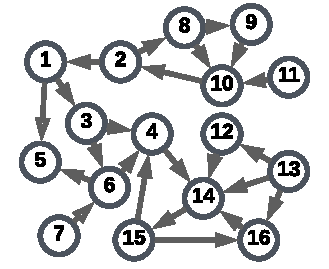
\includegraphics[width=0.23\linewidth]{out/about-frontier-11.pdf}
  }
  \subfigure[Marking initial affected vertices (DF)]{
    \label{fig:about-frontier-df2}
    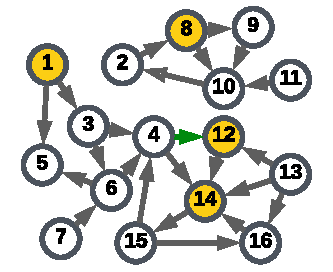
\includegraphics[width=0.23\linewidth]{out/about-frontier-32.pdf}
  }
  \subfigure[After first iteration (DF)]{
    \label{fig:about-frontier-df3}
    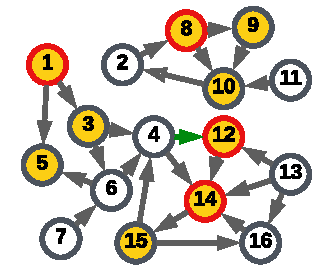
\includegraphics[width=0.23\linewidth]{out/about-frontier-33.pdf}
  }
  \subfigure[After second iteration (DF)]{
    \label{fig:about-frontier-df4}
    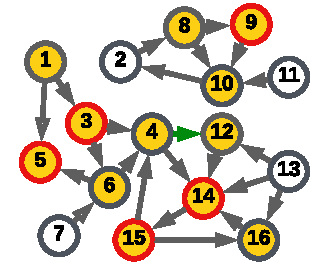
\includegraphics[width=0.23\linewidth]{out/about-frontier-34.pdf}
  } \\[2ex]
  \subfigure[Initial graph]{
    \label{fig:about-frontier-dfp1}
    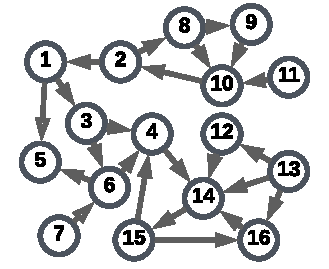
\includegraphics[width=0.23\linewidth]{out/about-frontier-11.pdf}
  }
  \subfigure[Marking initial affected vertices (DF-P)]{
    \label{fig:about-frontier-dfp2}
    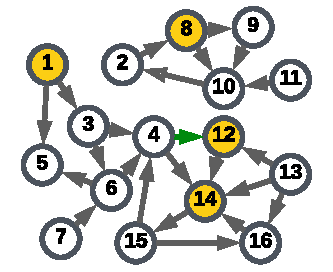
\includegraphics[width=0.23\linewidth]{out/about-frontier-32.pdf}
  }
  \subfigure[After first iteration (DF-P)]{
    \label{fig:about-frontier-dfp3}
    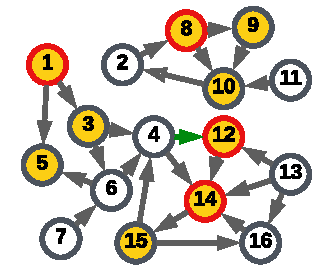
\includegraphics[width=0.23\linewidth]{out/about-frontier-33.pdf}
  }
  \subfigure[After second iteration (DF-P)]{
    \label{fig:about-frontier-dfp4}
    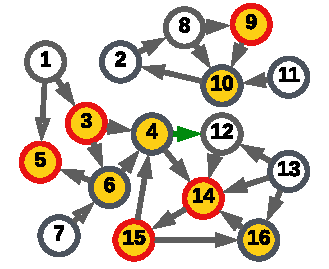
\includegraphics[width=0.23\linewidth]{out/about-frontier-44.pdf}
  } \\[2ex]
  \subfigure[Initial graph]{
    \label{fig:about-frontier-dt1}
    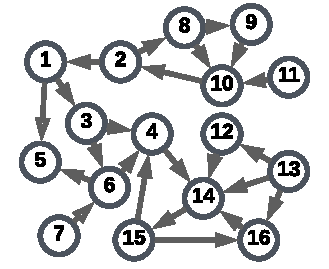
\includegraphics[width=0.23\linewidth]{out/about-frontier-11.pdf}
  }
  \subfigure[Marking affected vertices (DT)]{
    \label{fig:about-frontier-dt2}
    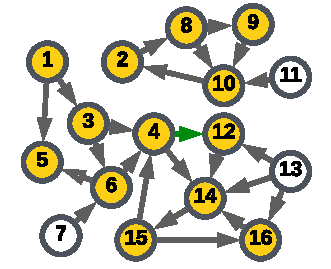
\includegraphics[width=0.23\linewidth]{out/about-frontier-22.pdf}
  }
  \subfigure[After first iteration (DT)]{
    \label{fig:about-frontier-dt3}
    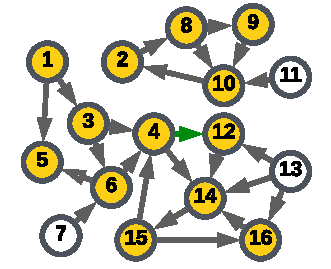
\includegraphics[width=0.23\linewidth]{out/about-frontier-22.pdf}
  }
  \subfigure[After second iteration (DT)]{
    \label{fig:about-frontier-dt4}
    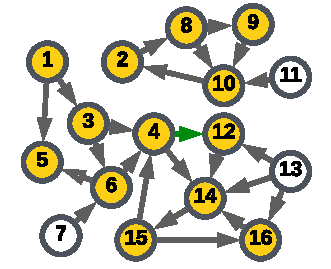
\includegraphics[width=0.23\linewidth]{out/about-frontier-22.pdf}
  } \\[-2ex]
  \caption{An example showcasing our improved \textit{Dynamic Frontier (DF)} and \textit{Dynamic Frontier with Pruning (DF-P)} approaches, in subfigures (a)-(d) and (e)-(h) respectively, in contrast to the \textit{Dynamic Traversal (DT)} approach, shown in subfigures (i)-(l).}
  \label{fig:about-frontier}
\end{figure*}

\ignore{An example showcasing our improved \textit{Dynamic Frontier (DF)} and \textit{Dynamic Frontier with Pruning (DF-P)} approaches. The initial graph has $16$ vertices and $23$ edges. The graph is updated with an edge insertion $(4, 12)$ and an edge deletion $(2, 1)$. Consequently, with DF and DF-P PageRank, the outgoing neighbors of vertices $2$ and $4$ (i.e., vertices $1$, $8$, $12$, and $14$) are marked as affected (shown with yellow fill). In the first iteration, when computing the ranks of these affected vertices, it is observed that the relative change in rank of vertices $1$, $8$, $12$, and $14$ exceeds the frontier tolerance $\tau_f$ (indicated with a red border). Therefore, their outgoing neighbors (i.e., vertices $3$, $5$, $9$, $10$, $14$, and $15$) are also marked as affected, with both DF and DF-P PageRank. In the second iteration, the relative rank change of vertices $3$, $5$, $9$, $14$, and $15$ surpasses the frontier tolerance $\tau_f$, resulting in their outgoing neighbors (i.e., vertices $4$, $6$, $10$, $15$, and $16$) being marked as affected. Additionally, with DF-P PageRank, vertices $1$, $8$, and $12$ are no longer marked as affected as their relative rank change falls below prune tolerance $\tau_p$. In the following iteration, the rankings of affected vertices are updated once more. If the rank change of each vertex falls within the iteration tolerance $\tau$, indicating convergence, the algorithm terminates. In contrast, the \textit{Dynamic Traversal (DT)} approach, marks all vertices reachable from $2$ and $4$ as affected. The ranks of this set of affected vertices are then updated in each iteration.}


In the second iteration, as illustrated in Figures \ref{fig:about-frontier-df4} and \ref{fig:about-frontier-dfp4}, another round of updates is applied to the ranks of the impacted vertices. Notably, the ranks of vertices $3$, $5$, $9$, $14$, and $15$ exhibit a relative change exceeding the designated frontier tolerance $\tau_f$. Consequently, employing DF/DF-P PageRank, we identify the outgoing neighbors of these vertices, namely vertices $4$, $6$, $10$, $15$, and $16$, as affected. Conversely, the relative change in rank of vertices $1$, $8$, and $12$ remains below the prune tolerance threshold $\tau_p$. Consequently, utilizing DF-P PageRank, these vertices are no longer classified as affected, indicating a probable convergence of their ranks. This action effectively contracts the frontier of affected vertices. However, if a vertex's rank has not yet converged, it might be re-designated as affected by one of its in-neighbors. Subsequently, in the ensuing iteration, the ranks of affected vertices undergo further updates. Should the change in rank for each vertex fall within the defined iteration tolerance $\tau$\ignore{(we use $L\infty$-norm for convergence detection)}, it signifies convergence of the ranks, and the algorithm halts.

\paragraph{Contrasting with Dynamic Traversal (DT) PageRank:}

We now compare DF and DF-P PageRank with DT PageRank (see Figures \ref{fig:about-frontier-dt1}-\ref{fig:about-frontier-dt4}). In Figure \ref{fig:about-frontier-dt2}, the identical batch update applied to the original graph is depicted, akin to Figures \ref{fig:about-frontier-df2} and \ref{fig:about-frontier-dfp2}. In response to this update, DT PageRank designates all vertices reachable from $2$ and $4$ as affected, i.e., all vertices except $7$, $11$, and $13$. Subsequently, the ranks of this subset of affected vertices undergo updates in each iteration\ignore{(while the ranks of unaffected vertices remain unchanged)}, continuing until convergence is achieved.

%% Describe how you determing the correct partitioning approach




\subsection{Determining suitable Partitioning approach}
\label{sec:parition-determine}

We first need to determine a suitable approach for frontier expansion, and an associate frontier tolerance $\tau_f$ value that allows us to minimize processed vertices, while limiting error to that of ranks obtained with Static PageRank using the same iteration tolerance $\tau$. For this, we experiment with three approaches. These include marking neighbors of a vertex as affected, based on change in rank of the vertex $\Delta r$, change in its contribution factor $\Delta r/d$, or relative change in its rank $\Delta r/r$. Here, $\Delta r$ is the rank change, $d$ is the out-degree, and $r$ is the \texttt{max} of its previous and current rank values.

For $\Delta r$ and $\Delta r/d$, we adjust $\tau_f$ from $\tau$ to $\tau/10^5$; and for $\Delta r/r$, we adjust it from $0.1$ to $10^{-6}$. This is done on real-world dynamic graphs, shown in Table \ref{tab:dataset}, with batch updates of size $10^{-5}|E_T|$. Outgoing neighbors are marked affected if the respective measure exceeds $\tau_f$. Figure \ref{fig:adjust-frontier} shows the mean speedup (with respect to Static PageRank) and rank error (compared to ranks obtained with reference Static PageRank) with each approach for frontier expansion. Results indicate that the $\Delta r/r$ approach with a $\tau_f$ of $10^{-6}$ performs best, while yielding lower error than Static PageRank.

\begin{figure}[!hbt]
  \centering
  \subfigure{
    \label{fig:adjust-partition--all}
    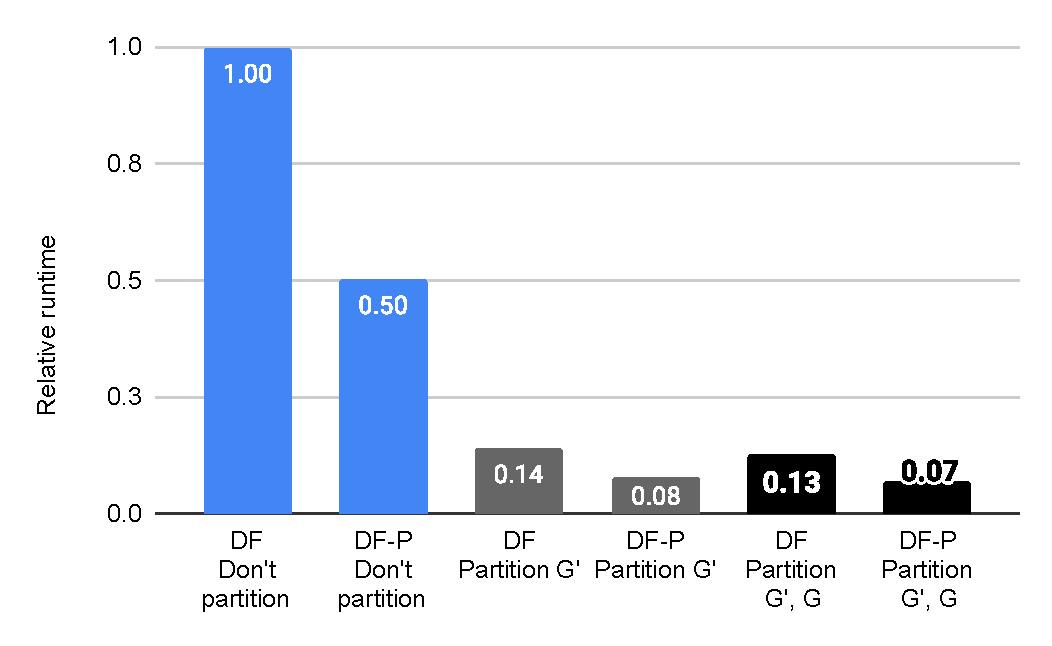
\includegraphics[width=0.98\linewidth]{out/adjust-partition.pdf}
  } \\[-2ex]
  \caption{Mean relative runtime with our \textit{Dynamic Frontier (DF)} and \textit{Dynamic Frontier with Pruning (DF-P)} approaches across three different levels of work-partitioning for GPU computation. Here, \textit{Partition $G$} denotes partitioning the vertices of the current graph $G$ by their out-degree, while \textit{Partition $G'$} signifies partitioning the vertices by their in-degree. Note that $G'$ stands for the transpose of the current graph $G$.}
  \label{fig:adjust-partition}
\end{figure}

\begin{algorithm}[!hbt]
\caption{Our GPU-based Dynamic Frontier (DF*) PageRank.}
\label{alg:frontier}
\begin{algorithmic}[1]
\Require{$G^t(V^t, E^t), G^{t'}$: Current input graph, and its transpose}
\Require{$\Delta^{t-}, \Delta^{t+}$: Edge deletions and insertions (input)}
\Require{$R^{t-1}$: Previous rank vector}
\Require{$R, R_{new}$: Rank vector in the previous, current iteration}
\Ensure{$\delta_V, \delta_N$: Is a vertex, or neighbors of a vertex affected}
\Ensure{$P, P'$: Partitioned vertex IDs --- low out-, in-degree first }
\Ensure{$N_P, N'_P$: Number of vertices with low out-, in-degree}
\Ensure{$\Delta R$: $L\infty$-norm between previous and current ranks}
\Ensure{$\tau$: Iteration tolerance}

\Statex

\Function{dynamicFrontier}{$G^t, G^{t'}, \Delta^{t-}, \Delta^{t+}, R^{t-1}$}
  \State $\rhd$ Initialize ranks
  \State $R \gets R_{new} \gets R^{t-1}$ \label{alg:frontier--initialize}
  \State $\rhd$ Partition vertex IDs by out- and in-degree 
  \State $\{P, N_P\} \gets partition(G^t)$
  \State $\{P', N'_P\} \gets partition(G^{t'})$
  \State $\rhd$ Mark initial set of affected vertices
  \State $\{\delta_V, \delta_N\} \gets initialAffected(G^t, \Delta^{t-}, \Delta^{t+})$
  \State $expandAffected(\delta_V, \delta_N, G^t, P, N_P)$
  \State $\rhd$ Perform PageRank iterations
  \ForAll{$i \in [0 .. MAX\_ITERATIONS)$} \label{alg:frontier--compute-begin}
    \State $\delta_N \gets \{\}$
    \State $updateRanks(\delta_V, \delta_N, R_{new}, R, G^t, P', N'_P)$
    \State $\Delta R \gets l_{\infty}NormDelta(R_{new}, R)$ \textbf{;} $swap(R_{new}, R)$
    \If{$\Delta R \leq \tau$} \textbf{break}
    \EndIf
    \State $expandAffected(\delta_V, \delta_N, G^t, P, N_P)$
  \EndFor \label{alg:frontier--compute-end}
  \State \ReturnInline{$R$} \label{alg:frontier--return}
\EndFunction
\end{algorithmic}
\end{algorithm}





\subsection{Determination of Prune tolerance ($\tau_p$)}
\label{sec:prune-tolerance}

We now embark on determining a suitable value for the prune tolerance $\tau_p$ to complement the optimal frontier expansion approach $\Delta r/r$, which employs a frontier tolerance $\tau_f$ of $10^{-6}$ as identified in Section \ref{sec:frontier-tolerance}. This entails adjusting $\tau_p$ from $\tau_f$ to $\tau_f/10^4$. Additionally, to err on the side of caution, we explore the effects of lower $\tau_f$ values, namely $10^{-7}$ and $10^{-8}$. These experiments are conducted on real-world graphs, employing batch updates of size $10^{-5}|E_T|$ as outlined earlier. A vertex is categorized as unaffected if its relative rank change $\Delta r/r$ falls within the designated $\tau_p$ range.

Figure \ref{fig:adjust-prune} presents the mean speedup, compared to Static PageRank, and the corresponding rank error observed when employing different $\tau_f$ values for frontier expansion. The rank error is measured with respect to reference Static PageRank, as discussed in Section \ref{sec:measurement}. Notably, the results highlight that the $\Delta r/r$ approach, particularly with a $\tau_f$ set to $10^{-6}$ and an accompanying $\tau_p$ of $\tau_f = 10^{-6}$, achieves superior performance by attaining lower rank error compared to Static PageRank.




\subsection{Our DF* PageRank implementation}

Algorithm \ref{alg:frontier} shows the pseudocode of our improved Dynamic Frontier (DF) and Dynamic Frontier with Pruning (DF-P) PageRank. It takes as input the previous $G^{t-1}$ and current $G^t$ snapshot of the graph, edge deletions $\Delta^{t-}$ and insertions $\Delta^{t+}$ in the batch update, the previous rank vector $R^{t-1}$, and returns the updated ranks $R$.

The algorithm begins by initializing the current rank vector $R$ with the previous rank vector $R^{t-1}$ (line \ref{alg:frontier--initialize}), and marking the initially affected vertices based on edge deletions $\Delta^{t-}$ and insertions $\Delta^{t+}$ in parallel (lines \ref{alg:frontier--mark-begin}-\ref{alg:frontier--mark-end}). It then iteratively computes the rank $R[v]$ for each affected vertex $v$ (lines \ref{alg:frontier--compute-begin}-\ref{alg:frontier--compute-end}). This computation is performed in parallel, considering the incoming edges $G^t.in(v)$. Depending on whether DF or DF-P PageRank is selected, the corresponding formula for rank calculation is applied (lines \ref{alg:frontier--formula-begin}-\ref{alg:frontier--formula-end}). The algorithm then checks if the relative change in rank $\Delta r / \max(r, R[v])$ exceeds the frontier tolerance $\tau_f$, marking out-neighbor vertices as affected if so. Additionally, with DF-P PageRank, if the relative change in rank lies within the prune tolerance $\tau_p$, the vertex $v$ is marked as not affected. The iteration continues until either the maximum change in ranks $\Delta R$ falls below the iteration tolerance $\tau$, or the maximum number of iterations $MAX\_ITERATIONS$ is reached. Finally, the algorithm returns the final rank vector $R$ (line \ref{alg:frontier--return}).

In a push-based approach for PageRank computation, each thread calculates and sums the outgoing PageRank contribution of its vertex to its neighbors, necessitating atomic updates. In contrast, with a pull-based approach, each vertex's rank is updated through a single write by a thread \cite{verstraaten2015quantifying}. We find this to be more efficient and employ it for all implementations. Furthermore, we employ an asynchronous implementation of DF and DF-P PageRank, using a single rank vector, for potentially faster convergence and elimination of memory copies for unaffected vertices. This, based on our previous research \cite{sahu2024incrementally}, outperforms synchronous implementations, especially with smaller batch sizes. We also utilize asynchronous implementations for Naive-dynamic (ND) and Dynamic Traversal (DT) PageRank, but not for Static PageRank (async not faster).
